%%%%%%%% ICML 2020 EXAMPLE LATEX SUBMISSION FILE %%%%%%%%%%%%%%%%%

\documentclass{article}

% Recommended, but optional, packages for figures and better typesetting:
\usepackage{microtype}
\usepackage{graphicx}
\usepackage{subfigure}
\usepackage{booktabs} % for professional tables

% hyperref makes hyperlinks in the resulting PDF.
% If your build breaks (sometimes temporarily if a hyperlink spans a page)
% please comment out the following usepackage line and replace
% \usepackage{icml2020} with \usepackage[nohyperref]{icml2020} above.
\usepackage{hyperref}

% Attempt to make hyperref and algorithmic work together better:
\newcommand{\theHalgorithm}{\arabic{algorithm}}

% Use the following line for the initial blind version submitted for review:
%\usepackage{icml2020}

% OUR PACKAGES
\usepackage{amssymb}
\usepackage{amsbsy}
\usepackage{amsmath}
%\usepackage{breqn}
\def\bx{\mathbf{x}}
\def\bX{\mathbf{X}}
\def\bz{\mathbf{z}}
\def\bZ{\mathbf{Z}}
\usepackage{amsthm}
\newtheorem{thm}{Theorem}[section] % reset theorem numbering for each chapter
\theoremstyle{plain}
\newtheorem{assumption}{Assumption}[section]
\theoremstyle{definition}
\newtheorem{defn}[thm]{Definition} % definition numbers are dependent on theorem numbers
\newtheorem{exmp}[thm]{Example} % same for example numbers
\newtheorem{lemma}[thm]{Lemma}
\newtheorem{remark}[thm]{Remark}

% If accepted, instead use the following line for the camera-ready submission:
\usepackage[accepted]{icml2020}

% The \icmltitle you define below is probably too long as a header.
% Therefore, a short form for the running title is supplied here:
\icmltitlerunning{Robust Variational Autoencoder for Tabular Data with $\beta$ Divergence}

\begin{document}

\twocolumn[
\icmltitle{Robust Variational Autoencoder for Tabular Data with $\beta$ Divergence}

% It is OKAY to include author information, even for blind
% submissions: the style file will automatically remove it for you
% unless you've provided the [accepted] option to the icml2020
% package.

% List of affiliations: The first argument should be a (short)
% identifier you will use later to specify author affiliations
% Academic affiliations should list Department, University, City, Region, Country
% Industry affiliations should list Company, City, Region, Country

% You can specify symbols, otherwise they are numbered in order.
% Ideally, you should not use this facility. Affiliations will be numbered
% in order of appearance and this is the preferred way.
%\icmlsetsymbol{equal}{*}

\begin{icmlauthorlist}
\icmlauthor{Sergul Aydore}{aws}
\icmlauthor{Haleh Akrami}{usc}
\icmlauthor{Richrd M. Leahy}{usc}
\icmlauthor{Anand A. Joshi}{usc}
\end{icmlauthorlist}

\icmlaffiliation{aws}{Amazon Web Service, New York, USA}
\icmlaffiliation{usc}{Signal and Image Processing Institute, University of Southern California, USA}

\icmlcorrespondingauthor{Sergul Aydore}{sergulaydore@gmail.com}
\icmlcorrespondingauthor{Haleh Akrami}{akrami@usc.edu}

% You may provide any keywords that you
% find helpful for describing your paper; these are used to populate
% the "keywords" metadata in the PDF but will not be shown in the document
\icmlkeywords{Machine Learning, ICML}

\vskip 0.3in
]

% this must go after the closing bracket ] following \twocolumn[ ...

% This command actually creates the footnote in the first column
% listing the affiliations and the copyright notice.
% The command takes one argument, which is text to display at the start of the footnote.
% The \icmlEqualContribution command is standard text for equal contribution.
% Remove it (just {}) if you do not need this facility.

\printAffiliationsAndNotice{}  % leave blank if no need to mention equal contribution
%\printAffiliationsAndNotice{\icmlEqualContribution} % otherwise use the standard text.

\begin{abstract}
We propose the robust variational autoencoder with $\beta$ divergence for tabular data (RTVAE) with mixed categorical and continuous features. Variational autoencoders (VAE) and their variations are popular frameworks for anomaly detection problems. The primary assumption is that we can learn representations for normal patterns via VAEs and any deviation from that can indicate anomalies. However, the training data itself can contain outliers. The source of outliers in training data can be either data collection process itself (random noise) or a malicious attacker (data poisoning) who may target to degrade the performance of the machine learning model. In either case, these outliers can disproportionately affect the training process of VAEs and may lead to wrong conclusions about what the normal behavior is. In this work, we derive a novel form of a variational autoencoder for tabular data sets with categorical and continuous features that is robust to outliers in training data. Our results on the anomaly detection application for network traffic datasets demonstrate the effectiveness of our approach.
\end{abstract}

\section{Introduction}
\label{sec:introduction}
Anomaly is defined as an observation that does not conform to normal patterns in the data. Anomalies can indicate a previously unknown mechanism that arouses suspicion. Early detection of anomalies is crucial for decision making systems to ensure undisrupted business. Anomaly detection is used in a wide variety of applications such as fraud and intrusion detection, military surveillance and medical diagnosis \cite{chandola2007outlier}. Our motivating application in this work is detecting malicious activities from network traffic data that compromise both categorical and continous features.

Due to limited labeled data, unsupervised machine learning algorithms such as one-class SVM \cite{erfani2016high}, K-Means \cite{munz2007traffic}, principal component analysis (PCA) \cite{chandola2007outlier} and variational autoencoders (VAEs) \cite{an2015variational,yao2019unsupervised} are adopted for anomaly detection problems. These methods are based on intrinsic properties of the dataset and do not require any labels.Their core idea is to learn the representations in the original or some latent feature space and then detect anomalies by computing the deviation from normal patterns. Among these methods, spectral anomaly detection approaches such as PCAs and autoencoders try to find lower dimensional representations of the original data\cite{an2015variational}. It is believed that anomalies and normal data are separable in this low dimensional representations. Once lower dimensional representations are learned, the data is reconstructed back in the original dimension. Reconstruction error between the original data and reconstructed data is used as a score to detect anomalies.Autoencoder and its variations are the core of all Unsupervised deep anomaly detection. These models are also used for learning low representations by stacking up layers that forms deep neural networks.

VAEs \cite{kingma2013auto} are generative models that adopt variational inference and graphical models. The advantage of VAE over PCA and autoencoder is that it can learn the distribution of the data that provides a reconstruction probability in addition to reconstruction error as the anomaly score \cite{an2015variational}. VAE has two components: an encoder and a decoder. The encoder transforms high dimensional data in a low-dimensional latent space with an approximate tractable posterior distribution. The decoder samples from this distribution and transforms the sample back to the original dimension. The VAE minimizes two terms: the reconstruction cost and the regularizer. The regularizer penalizes any discrepancy between the prior distribution of the latent representations and the distribution induced by the encoder. 

The main assumption behind the use of latent space representations is that the training data is clean and represents normal behavior. However, in practice, training data can inevitably contain outliers or anomalies.The presence of outliers can have a disproportionate impact on training due to large negative log-likelihood values. Hence, not only that the model's representation of normal behavior degrade but also it may treat outliers as normal samples during inference. Therefore, achieving robustness to outliers is crucial in unsupervised models for accurate detection of outliers.

\subsection{Our Contribution}
Our work can be viewed as an extension of \citet{akrami2019robust} to tabular data. In order to achieve robustness to outliers, Previous approaches
focus on modification of network architectures, adding constraints or modeling of outlier distribution\cite{zhai2017robust,eduardo2019robust}. In contrast,  \citet{akrami2019robust}  adopt $\beta$-divergence from robust statistics \cite{futami2017variational}. The log-likelihood term that VAE uses in reconstruction loss minimizes the KL-divergence between the empirical distribution of the data and the parametric distribution at the output of the decoder. After demonstrating the non-robustness of the KL divergence, \citet{akrami2019robust} replaced the KL-divergence for data fitting to a robust $\beta$-divergence \cite{basu1998robust}. However, their derivations and implementations were limited to images. In this work, we derive formulation for categorical variables and propose a training mechanism for tabular datasets.We show that the proposed approach works more accurately than the standard VAE using the publicly available tabular network traffic datasets.

%\subsection{Related Work}
%Recently, \cite{beggel2019robust} proposed to use adversarial autoencoders (AAEs) to achieve robustness to outliers. The main difference between VAE and AAE is that AAE has additional adversarial training criterion. However, this approach requires pre-training, refinement and re-training steps which is not practical for our purposes. \citet{zhou2017anomaly} proposed robust deep autoencoders inspired by robust PCA \cite{candes2011robust}. The idea is simply to split the input into two components: $L_D$ and $S$ where $L_D$ can be learned by an autoencoder and $S$ contains the outliers and noise in the data. However, this approach is not probabilistic and does not extend to generative models.


%\subsection{Motivation via a Toy Example}
%In order to illustrate our motivation on using $\beta$-divergence as opposed to KL-divergence, we run simple simulations illustrated in Figure \ref{fig:simulations_compare_KL_with_beta}. Here, we sampled from a distribution $p$ which is a mixture of two Gaussian distributions where the tall mode represents normal samples and the short mode indicates the presence of outliers. Our goal is to learn a single-mode Gaussian distribution $q_{\theta}$. We minimize KL and $\beta$ divergences separately to optimize $\theta$. Figure \ref{fig:simulations_compare_KL_with_beta} shows the estimated distributions after optimizing these two divergences. The estimated distribution computed from optimizing $\beta$-divergence is robust to the outliers whereas the distribution estimated using KL-divergence attempts to also account for the presence of outliers.
%
%\begin{figure}[h!]
%	\centering
%	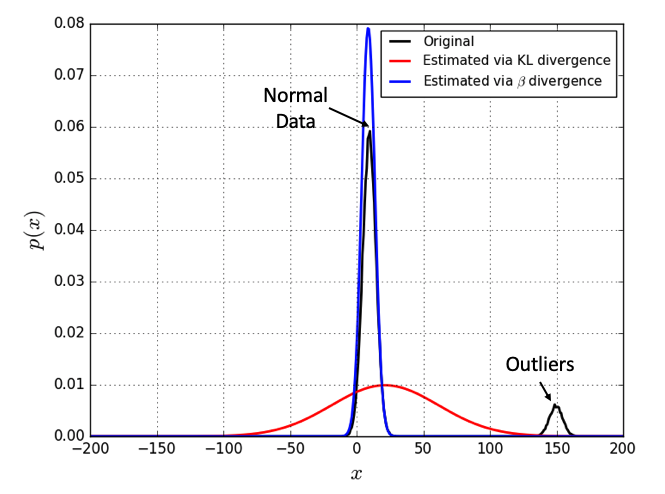
\includegraphics[scale=0.3]{./figures/simulations_compare_KL_with_beta.png}
%	\caption{Illustration of robustness of $\beta$-divergence to outliers: optimizing KL-divergence for parameter estimation of Gaussian distribution attempts to also account for the presence of outliers, whereas optimizing $\beta$-divergence results in an estimate that is more robust to outliers.}	
%	\label{fig:simulations_compare_KL_with_beta}
%\end{figure}

\section{Variational Autoencoders}
\label{sec:variational_autoencoders}
In this section, we provide a review for VAEs. We adopt the notation in \citet{ghosh2019variational}. Let $\mathcal{X} = \left\{ \bx_i \right\}_{i=1}^N$ be high-dimensional i.i.d. samples drawn from the true data distribution $p_{\textrm{data}}(\bx)$ over a random variable $\bX$. Generative modeling aims to learn a mechanism from $\mathcal{X}$ to draw new samples such that $\bx_{\textrm{new}} \sim p_{\textrm{data}}$. VAEs provide a framework to achieve this goal by learning representation in low-dimensional latent space. The generative process of the VAE is defined as
\begin{equation}
\bz_{\textrm{new}} \sim p(\bZ) \quad \quad \quad \bx_{\textrm{new}} \sim p_{\theta}(\bX | \bZ = \bz_{\textrm{new}})
\end{equation}
where $p(\bZ)$ is a fixed prior distribution over latent space $\bZ$. A stochastic decoder
\begin{equation}
D_{\theta}(\bz) = \bx \sim p_{\theta}(\bx \mid \bz) = p(\bX | g_{\theta}(\bz))
\end{equation}
maps the latent variable to the input space via the \textit{likelihood} distribution $p_{\theta}$, where $g_{\theta}$ is a non-linear function, typically a neural network, parameterized by $\theta$. Consequently, a VAE estimates $p_{\textrm{data}}(\bx)$ as the infinite mixture model $p_{\theta}(\bx) = \int p_{\theta}(\bx \mid \bz) p(\bz) d\bz$. At the same time, the input space is mapped to the latent space via a stochastic encoder
\begin{equation}
E_{\phi}(\bx) = \bz \sim q_{\phi}(\bz \mid \bx) = q(\bZ \mid f_{\phi}(\bx))
\end{equation}
where $q_{\phi}(\bz \mid \bx)$ is the \textit{posterior} distribution given by another non-linear function $f_{\phi}$ parameterized by $\phi$.

Computing the marginal log-likelihood $\log p_{\theta}(\bx)$ is generally intractable. Therefore, it is common to follow a variational approach which focuses on maximizing the evidence lower bound (ELBO) for a sample  $\bx$:
\begin{equation}
\begin{split}
\log  &p_{\theta}(\bx) \geq  \textrm{ELBO}(\phi, \theta, \bx) \\
&= \mathbb{E}_{\bz \sim q_{\phi}(\bz \mid \bx)} \log p_{\theta}(\bx \mid \bz) - \mathbb{KL}(q_{\phi}(\bz \mid \bx) || p(\bz)) \\
&\triangleq -\mathcal{L}_{\textrm{ELBO}}
\end{split}
\label{eqn:elbo}
\end{equation}
Maximizing RHS of equation \ref{eqn:elbo} over data $\mathcal{X}$ with respect to parameters $\phi$ and $\theta$ corresponds to minimizing the loss
\begin{eqnarray}
\arg \min_{\phi, \theta} && \mathbb{E}_{\bx \sim p_{\textrm{data}}}  \mathcal{L}_{\textrm{ELBO}} \\
&=& \mathbb{E}_{\bx \sim p_{\textrm{data}}} \left[ \mathcal{L}_{\textrm{REC}} + \mathcal{L}_{\textrm{KL}} \right]
\end{eqnarray}
where $\mathcal{L}_{\textrm{REC}}$ and $\mathcal{L}_{\textrm{KL}}$ are defined for sample $\bx$ as follows:
\begin{eqnarray}
\mathcal{L}_{\textrm{REC}} &=& - \mathbb{E}_{\bz \sim q_{\phi}(\bz \mid \bx)} \log p_{\theta}(\bx \mid \bz) \\
\mathcal{L}_{\textrm{KL}} &=& \mathbb{KL}(q_{\phi}(\bz \mid \bx) || p(\bz)).
\label{eqn:L_rec_kl}
\end{eqnarray}
The reconstruction loss $\mathcal{L}_{\textrm{REC}}$ computes the quality of encoded samples $\bx$ through $D_{\theta} \left( E_{\phi}(\bx) \right)$. The KL-divergence term $\mathcal{L}_{\textrm{KL}}$ measures the similarity between $q_{\phi}(\bz \mid \bx)$ and the prior $p(\bz)$ for each $\bz$. This KL-divergence term is also called the regularizer term since it acts as a regularizer during training \cite{hoffman2016elbo}.

\section{Robust Variational Inference}
In this section, we show how the reconstruction term $\mathcal{L}_{\textrm{REC}}$ can be modified using a robust divergence in order to make it more robust to outliers for categorical data. This approach was first proposed in \cite{akrami2019robust} for Gaussian and Bernoulli variables. Here, we will provide an extension for categorical  variables. 

Let empirical distribution of $\bX$ be
\begin{equation}
\hat{p}(\bX) = \frac{1}{N} \sum_{i=1}^N \delta(\bX, \bx_i)
\end{equation}
where $\delta$ is the Dirac delta function. The KL-divergence between this empirical distribution $\hat{p}(\bX)$ and $p_{\theta}(\bX | \bz)$ can be written as
\begin{equation}
\begin{split}
 & \mathbb{KL}\left(\hat{p}(\bX) || p_{\theta}(\bX | \bz)  \right) = \int \hat{p}(\bX) \log \frac{\hat{p}(\bX)}{p_{\theta}(\bX | \bz)} d \bX  \\
& \quad \quad = \textrm{const} - \int \hat{p}(\bX) \log p_{\theta} (\bX \mid \bz) d \bX  \\
& \quad \quad = \textrm{const} - \int \frac{1}{N} \sum_{i=1}^N \delta(\bX, \bx_i) \log p_{\theta}(\bX \mid \bz) d \bX \\
& \quad \quad = \textrm{const} - \frac{1}{N} \sum_{i=1}^N \log p_{\theta}(\bx_i \mid \bz)
\end{split}
\end{equation}
indicating that maximizing the log-likelihood of a sample $\bx_i$ is equivalent to minimizing KL-divergence between the empirical distribution and the generative distribution for one sample. Let the KL-divergence for a single sample $\bx_i$ be
\begin{equation}
\mathbb{KL}^i \triangleq -\frac{1}{N} \log p(\bx_i \mid \bz).
\end{equation}
Then, the reconstruction loss for a single sample can be written as
\begin{equation}
\mathcal{L}_{\textrm{REC}}^i = N \mathbb{E}_{\bz \sim q_{\phi}(\bz \mid \bx)} \left [ \mathbb{KL}^i \right ].
\end{equation}
The log-likelihood term $ \log p(\bx_i \mid \bz)$ in $\mathbb{KL}^i$ is sensitive to the outliers because the negative log-likelihood of low probability samples can be arbitrarily high. Rather than using KL-divergence, it is possible to choose a different divergence measure to quantify the similarity between $\hat{p}(\bX)$ and $p_{\theta} (\bX \mid \bz)$. We use $\beta$-divergence which is defined as
\begin{equation}
\begin{split}
\mathbb{D}_{\beta}(\hat{p}(\bX) ||  p_{\theta} (\bX & \mid \bz) = \\
 & \frac{1}{\beta} \int \hat{p}(\bX)^{\beta + 1} d \bX \\
&  - \frac{\beta + 1}{\beta} \int \hat{p}(\bX) p_{\theta}(\bX \mid \bz)^{\beta} d \bX \\
&  + \int p_{\theta}(\bX \mid \bz)^{\beta + 1} d \bX
\end{split}
\end{equation}
which converges to $\mathbb{KL}$ as $\beta \rightarrow 0$.  It can be shown that minimizing $\beta$-divergence is equivalent to minimizing $\beta$-cross-entropy \cite{eguchi2010entropy, futami2017variational} which is defined as
\begin{equation}
\begin{split}
\mathbb{H}_{\beta} & (\hat{p}(\bX) || p_{\theta}(\bX | \bz)) = \\
& - \frac{\beta + 1}{\beta} \int \hat{p}(\bX) \left(p_{\theta}(\bX | \bz)^{\beta}-1 \right) d \bX  \\ 
& \quad + \int p_{\theta}(\bX| \bz)^{\beta + 1} d \bX.
\end{split}
\label{eqn:beta_entropy}
\end{equation}

\begin{algorithm}[!b]
   \caption{Training RTVAE}
   
   \textbf{Input:} 
   
	\hspace{\parindent} Initialize the parameters of the encoder $q_{\phi}(\bz \mid \bx)$ and the decoder $p_{\theta}(\bx \mid \bz)$.
		
	\hspace{\parindent} Robust divergence coefficient $\beta \geq 0$.

   \textbf{Output:} 
	\hspace{\parindent} $\phi$, $\theta$

\begin{algorithmic}[1]
   \WHILE{$\phi$ and $\theta$ not converged}
      \STATE Initialize $\mathcal{L}_{\textrm{REC-}\beta}=0 $
   \STATE Sample $\{\bx_1, \cdots, \bx_N \}$ from the training set
   \STATE Sample $\{\bz_1, \cdots, \bz_N \}$ from the prior $p(\bz)$
   \STATE Sample $\{\tilde{\bz}_1, \cdots, \tilde{\bz}_N \}$ from $q_{\phi}(\bz \mid \bx_i)$
   \FOR {$j$ in features}
   \STATE Compute $\beta$-divergence term: 
	\IF   {$j$ is a categorical variable}
   \STATE $\mathcal{L}_{\textrm{REC-}\beta} += - \frac{\beta+1}{N \beta} \sum_{i=1}^N \left( p_{\theta}(\bx_i^j \mid \tilde{\bz}_i)^{\beta} - 1 \right)$ \\  \quad \quad  \quad \quad \quad $+ \sum_{k=1}^K p_{\theta}(\bX^j == k \mid \tilde{\bz}_i)^{\beta+1}$
   \ELSIF {$j$ is a continous variable}
   \STATE $\mathcal{L}_{\textrm{REC-}\beta} +=$ \\
    \quad $- \frac{\beta+1}{N \beta} \sum_{i=1}^N \frac{1}{(2 \pi \sigma^2)^{\beta/2}} \exp \left( - \frac{\beta}{2 \sigma^2} \| \hat{\bx}_i^j - \bx_i^j \|^2 \right)$ \\ \quad $+\frac{\beta + 1}{\beta}$
   \ENDIF
   \ENDFOR
   \STATE Compute the regularizer : \\\quad $\mathcal{L}_{\textrm{KL}} = \mathbb{KL}({q_{\phi}(\bz \mid \bx_i) || p(\bz)}) $
   \STATE Update $\phi$ and $\theta$ by descending the total loss \\\quad $\mathcal{L}_{\textrm{TOT}} = \mathcal{L}_{\textrm{REC-}\beta} + \mathcal{L}_{\textrm{KL}} $
   \ENDWHILE
   \STATE Return $\phi$, $\theta$
\end{algorithmic}
\label{alg:rvae}
\end{algorithm}

 \begin{figure*}[t!]
	\centering
	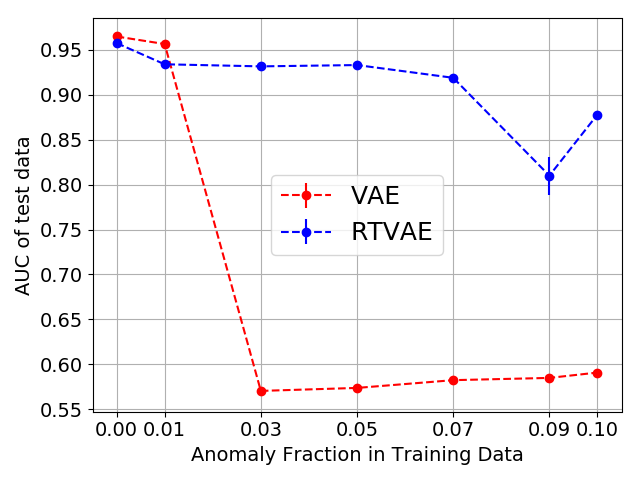
\includegraphics[scale=.33]{./figures/auc_original_kdd_regularizer_kld.png}
	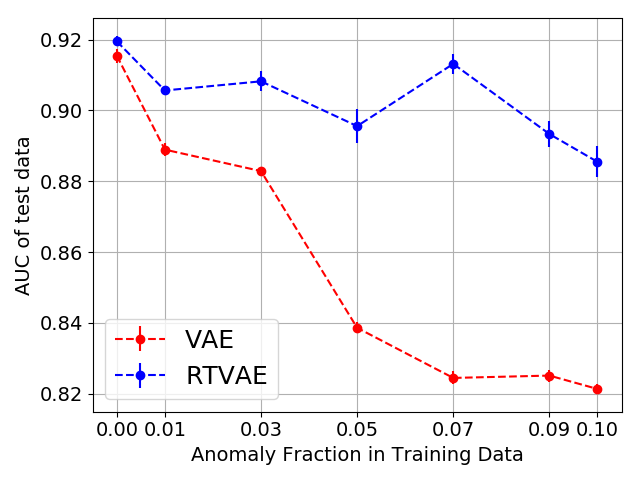
\includegraphics[scale=.33]{./figures/auc_kdd_regularizer_kld.png}
	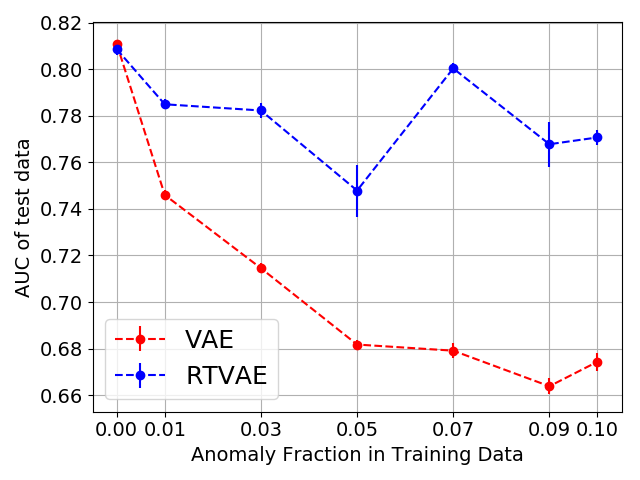
\includegraphics[scale=.33]{./figures/auc_UNSW_regularizer_kld.png}
	\caption{Performance comparison of VAE and RTVAE as function of contamination in training data for datasets KDDCup99 (left), NSLKDD (middle), and UNSW-NB15 (right)}.
	\label{fig:results}
\end{figure*}

Since we are interested in applying VAE to a categorical data, we can assume  that the generative distribution is a categorical distribution with $K$ categories. Then, the first integral in equation \ref{eqn:beta_entropy} becomes:
\begin{equation}
\begin{split}
\int \hat{p}(\bX) &  p_{\theta}(\bX | \bz)^{\beta }d \bX = \\
& \frac{1}{N} \int \sum_{i=1}^N \delta(\bX, \bx_i) \left( p_{\theta}(\bX | \bz)^{\beta} - 1 \right) d \bX   \\
&= \frac{1}{N} \sum_{i=1}^N  \left( p_{\theta}(\bx_i | \bz)^{\beta} - 1 \right)
\end{split}
\end{equation}
The second integral can be written as:
\begin{equation}
\begin{split}
\int p_{\theta}(\bX | & \bz)^{\beta + 1} dX = \\
& \int \prod_{k=1}^K p_{\theta}( \bX = k \mid \bz)^{\beta + 1} \delta (\bX, k) d \bX  \\
&= \sum_{k=1}^K p_{\theta}(\bX = k \mid \bz)^{\beta + 1}
\end{split}
\end{equation}
Let's define $\beta$-cross-entropy for a single point for a categorical variable as:
\begin{equation}
\begin{split}
\mathbb{H}_{\beta}^{i-\textrm{cat}} &= - \frac{\beta + 1}{\beta} \frac{1}{N} \left( p_{\theta}(\bx_i \mid \bz)^{\beta} - 1 \right) \\
& \quad \quad + \frac{1}{N} \sum_{k=1}^K p_{\theta}(\bX = k \mid \bz)^{\beta + 1}.
\end{split}
\end{equation}
Then, the reconstruction loss for a single categorical sample using $\beta$-divergence can be written as
\begin{equation}
\mathcal{L}_{\textrm{REC-} \beta}^i = N \mathbb{E}_{\bz \sim q_{\phi}(\bz \mid \bx)} \left [ \mathbb{H}_{\beta}^{i-\textrm{cat}} \right ].
\label{eqn:L_rec_beta_cat}
\end{equation}
We can use the formulation derived in \citet{akrami2019robust} for continuous variables with the assumption of Gaussian distribution for $p(\bx_i \mid \bz) = \mathcal{N}(\bx_i, \sigma)$ which leads to
\begin{equation}
\begin{split}
\mathbb{H} & _{\beta}^{i-\textrm{continous}} = \\
&- \frac{\beta + 1}{\beta} \frac{1}{N} \left( \frac{1}{(2 \pi \sigma^2)^{\beta/2}} \exp \left( - \frac{\beta}{2 \sigma^2} \| \hat{\bx}_i - \bx_i \|^2 \right) - 1 \right)
\end{split}
\end{equation}
where $\hat{\bx}_i$ is the output of the decoder and the reconstruction loss becomes
\begin{equation}
\mathcal{L}_{\textrm{REC-} \beta}^i = N \mathbb{E}_{\bz \sim q_{\phi}(\bz \mid \bx)} \left [ \mathbb{H}_{\beta}^{i-\textrm{continous}} \right ].
\label{eqn:L_rec_beta_continous}
\end{equation}

For a mixed type tabular data, we use either equation \ref{eqn:L_rec_beta_cat} or \ref{eqn:L_rec_beta_continous} depending on the type of the variable. We summarize the training of RTVAE in algorithm \ref{alg:rvae}.

\section{Experimental Results}
We compare the performance between regular VAE and our RTVAE by gradually contaminate the training dataset with more outliers to evaluate robustness to the outliers. We use three benchmark datasets made available by cyber security community: KDDCup 99, NSL-KDD and UNSW-NB15. The goal is to detect cyber attacks at the network level. All datasets are in tabular format with categorical and continuous columns. We measured the area under the receiver operating characteristic curve (AUC) as an evaluation metric. 

\textbf{KDDCup 99:} \cite{kdd99} is the dataset used for ``The Third Knowledge Discovery and Data Mining Tools'' competition. The task was to build an automated network intrusion detector that can distinguish between attacks and normal connections. There are 41 columns of which 8 of them are categorical. We use the complementary 
10 \% data for training and the labeled test data for testing.

\textbf{NSL-KDD:} \cite{nslkdd} is the refined version of KDDCup 99 to resolve some of the inherent problems in KDDCup 99 dataset. More specifically, the redundant connection records were removed to prevent detection models become biased towards frequent connection records. We used the available full training dataset for training and test dataset for testing.

\textbf{UNSW-NB15:} \cite{unsw} dataset was introduced by cyber security research team of Australian Centre for Cyber Security. We used the available partitioned datasets for training and testing. The data has 43 columns out of which, 9 features are categorical. 

\textbf{Implementation Details:} We use fully-connected neural networks both in encoder and decoder with \textrm{tanh} and \textrm{softmax} activation functions for continuous and categorical variables, respectively. We use Python 3.6 for implementation \cite{oliphant2007python} using he topen-source libraries PyTorch \cite{paszke2019pytorch}, scikit-learn \cite{pedregosa2011scikit},  and NumPy \cite{walt2011numpy}. We use Adam \cite{kingma2014adam} as an optimizer with learning rate $1e-3$ and bias correction parameters $0.5$ and $0.999$ for gradients and squared gradients, respectively. We vary the $\beta$ parameter from $1 e-5$ to $0.1$ in logarithmic scale. Model selection for $\beta$ and the early stopping was done based on the best AUC from the hold-out validation dataset (20 \% of the training dataset).

\textbf{Results:} The results in Figure \ref{fig:results} show that the performance of the vanilla VAE degrades significantly even with a small amount of contamination (1 \%). Our RTVAE, on the other hand, stays robust to the outliers in the training datasets.

\section{Conclusion}
We derived a formulation on how to use robust $\beta$ divergence in VAE framework for tabular datasets consisting of categorical and continuous features. Our results demonstrate that additional care needs to be taken when working with contaminated datasets with outliers and our RTVAE can provide such a care and robustness to outliers.  %Although, we use intrusion detection as an application, our work can be used in other anomaly detection applications using tabular datasets.
% In the unusual situation where you want a paper to appear in the
% references without citing it in the main text, use \nocite
\nocite{langley00}

\bibliography{mybib.bib}
\bibliographystyle{icml2020}




\end{document}


% This document was modified from the file originally made available by
% Pat Langley and Andrea Danyluk for ICML-2K. This version was created
% by Iain Murray in 2018, and modified by Alexandre Bouchard in
% 2019 and 2020. Previous contributors include Dan Roy, Lise Getoor and Tobias
% Scheffer, which was slightly modified from the 2010 version by
% Thorsten Joachims & Johannes Fuernkranz, slightly modified from the
% 2009 version by Kiri Wagstaff and Sam Roweis's 2008 version, which is
% slightly modified from Prasad Tadepalli's 2007 version which is a
% lightly changed version of the previous year's version by Andrew
% Moore, which was in turn edited from those of Kristian Kersting and
% Codrina Lauth. Alex Smola contributed to the algorithmic style files.
